\documentclass[12pt]{article}
\usepackage{light}
\usepackage{enumerate}

\newcommand{\Bob}{\mathcal{B}}
\newcommand{\Sandy}{\mathcal{S}}

%\hidesolutions
\showsolutions

\begin{document}

\recitation{19}{November 14, 2012}

\section*{Routes in a flood}

You want to walk from your house at $(0,0)$ to your friend Bob's house at $(n, n)$. Unfortunately, much of the city has been recently flooded, making some roads impassable. You and your friend were both lucky to escape! All the roads below the diagonal connecting you and your friend have been flooded.

\begin{center}
    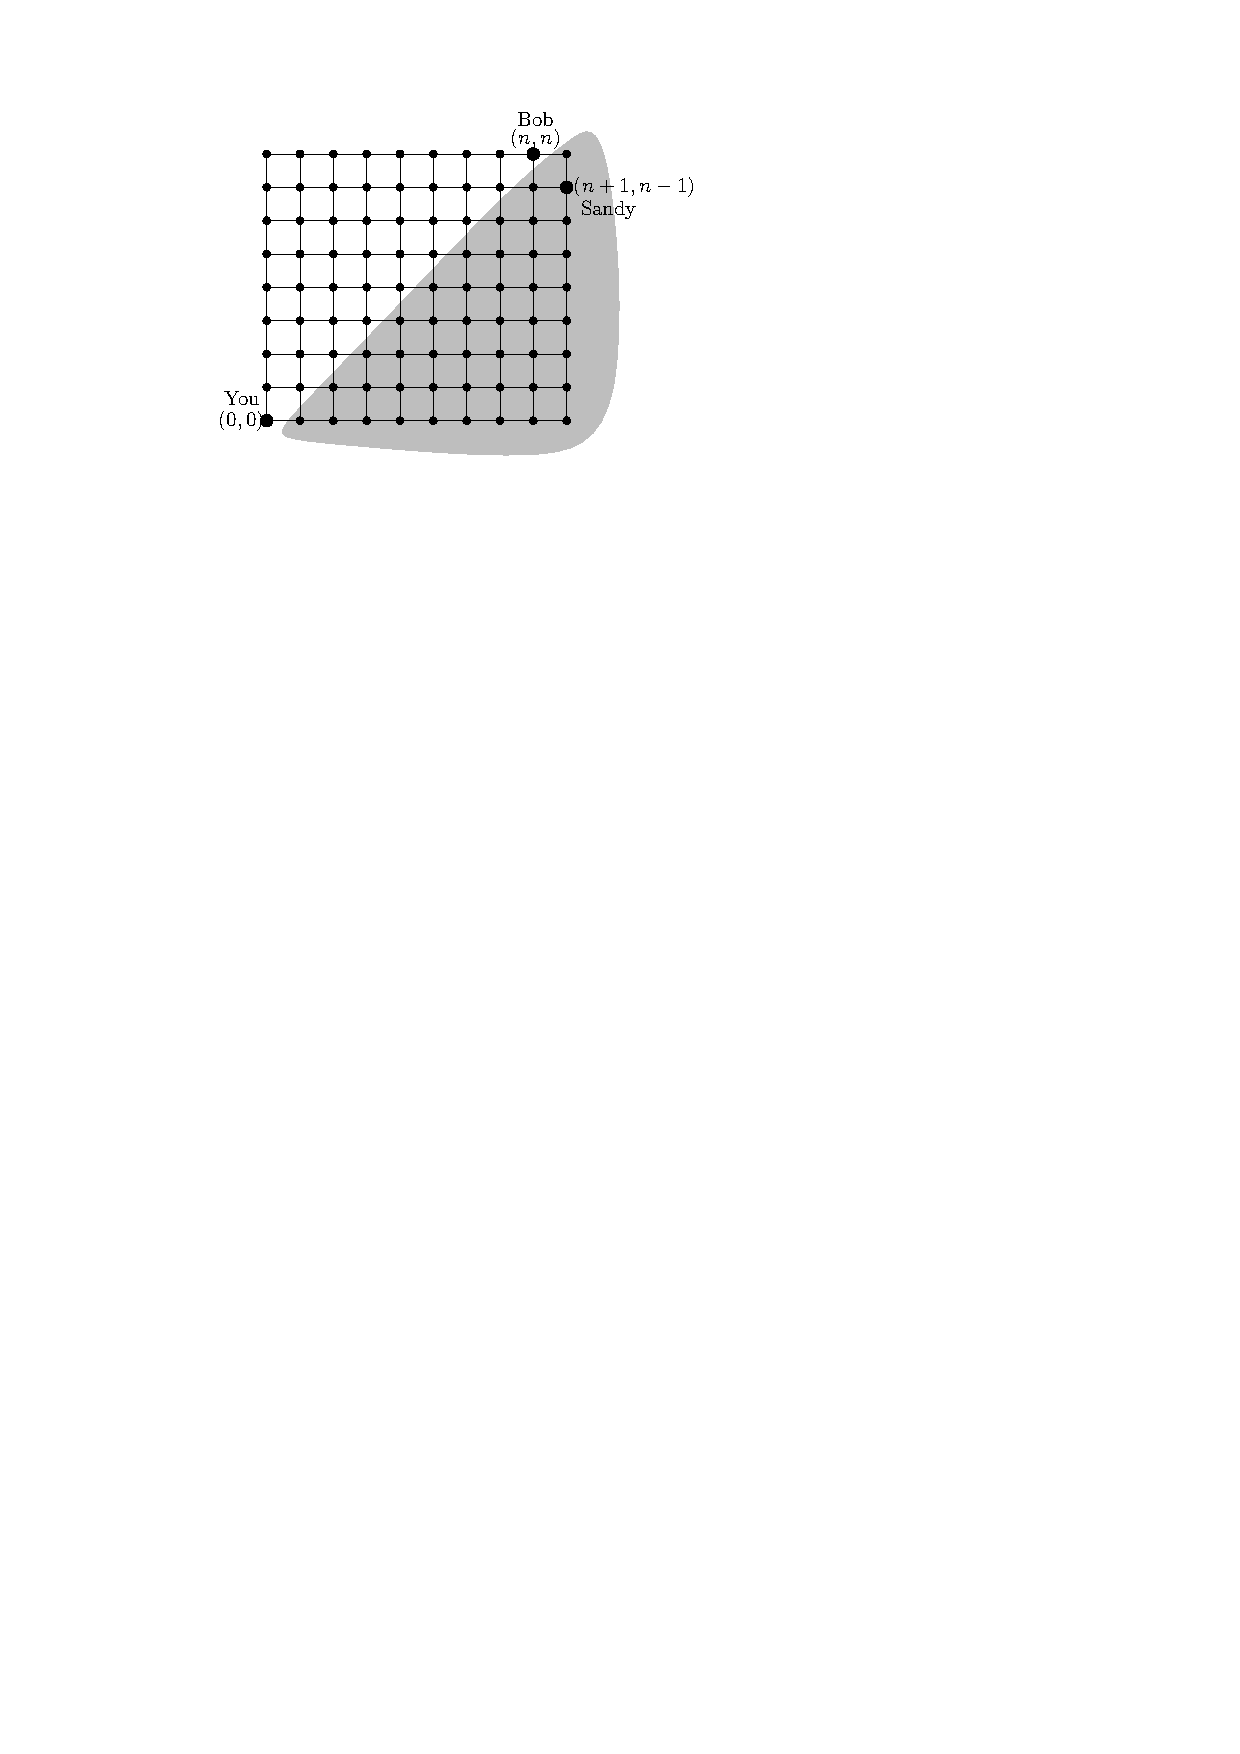
\includegraphics[page=1]{flooded}
\end{center}

We will answer the question: how many shortest paths are there to your friend's house? This is quite tricky, and involves a really beautiful bijection.

\begin{enumerate}[(a)]
    \item Let's begin with an easier problem. 

        You have another, less fortunate, friend living at coordinates $(n+1, n-1)$ on the map. 
        This friend (let's call her Sandy) is trapped in her apartment, and you want to bring her some supplies. Fortunately, you have a dinghy, and can traverse both flooded and unflooded roads.

        How many shortest paths are there to Sandy?

        \solution{This we saw in an earlier recitation; it is ${(n+1) + (n-1) \choose n + 1} = {2n \choose n+1}$, by the bijection to strings of length $2n$ containing $n-1$ N's and $n+1$ E's.}
        \newpage

    \item We will now count the number of shortest paths to Bob that \emph{do} involve at least one flooded road. This requires a very clever bijection, and is the real key to the argument. 

        To get you going, here is an example of the bijection; the path to Sandy is on the left, and the resulting path to Bob is on the right. Based on this, try to figure out the rule defining the bijection, and explain why it works. 
        Hence give the formula for the number of shortest paths to Bob involve at least one flooded road.

        \begin{figure}[h!]
            \centering
            \includegraphics[page=2]{flooded} \hspace{0.1cm}
            \includegraphics[page=3]{flooded}
        \end{figure}

        \solution{
            Let $\Bob$ be the set of shortest routes to Bob that involve at least one flooded road.
            Let $\Sandy$ denote the set of shortest routes to Sandy. 
            For any path $P \in \Sandy$, we define $f(P)$ as follows.
            Construct a new route that is the same as $P$, until the first flooded intersection. 
            From that point on, flip the route: for each step to the north in the original route $P$, take a step to the east, and for each step to the east in the original, take a step to the north.
            This resulting route is $f(P)$.

            First, let's observe that this new route $f(P)$ will end at $(n,n)$.
            The first flooded intersection will be at coordinates $(i + 1, i)$, for some $i$, since it's just below the diagonal.
            The rest of $P$ goes from $(i+1, i)$ to $(n + 1, n-1)$, so it moves $n - i$ steps east and $n-1-i$ steps north from $(i+1,i)$. After the flip, this becomes $n-1-i$ steps east and $n-i$ steps north, and so $f(P)$ will end at coordinates $(i + (n-i), i+1 + (n-1-i) = (n,n)$, as we wanted. It follows that $f(P) \in \Bob$, since also the route still involves at least one flooded intersection.

            The same idea shows that if we take a route $Q \in \Bob$, then flipping after the first flooded intersection yields a route $P$ from $(0,0)$ to $(n+1,n-1)$. So $P \in \Sandy$, and $f(P) = Q$. So $f$ is surjective. Moreover, $P$ is the only route so that $f(P)=Q$; so $f$ is injective.

            So $f$ is a bijection from $\Sandy$ to $\Bob$, and thus the number of routes to $(n,n)$ which use a flooded road is
            \[ |\Bob| = |\Sandy| = {2n \choose n+1}. \]
        }
        \newpage

\item So now you can answer the original question: how many shortest paths to Bob do not involve any flooded roads? 

    You should be able to simplify your answer down to the simple formula $\frac{1}{n+1}{2n \choose n}$. These numbers are known as \emph{Catalan numbers}.

    \solution[\vspace{4cm}]{
        The total number of paths (allowing flooded routes) is ${2n \choose n}$. Subtracting the paths that use a flooded road, we get
        \begin{align*}
            {2n \choose n} - {2n \choose n+1} &= \frac{(2n)!}{n!n!} - \frac{(2n)!}{(n+1)!(n-1)!}\\
                                              &= \frac{(2n)!}{(n!)^2}\left( 1 - \frac{n}{n+1}\right)\\
                                              &= \frac{1}{n+1}{2n \choose n}. 
        \end{align*}
    }

\end{enumerate}

\section*{Counting matching brackets} 

Catalan numbers appear all over the place. Consider the number of possible matched brackets of length $2n$. 
This is just a sequence of open and closed brackets, with $n$ open brackets and $n$ close brackets, where open and closed brackets are matched. 
For example, 
\[ ( \quad ( \quad ) \quad ( \quad ( \quad ) \quad ( \quad ) \quad ) \quad ) \]
is a matched bracket sequence of length $10$; but
\[ ( \quad ( \quad ) \quad ) \quad ( \quad ) \quad ) \quad ( \quad ( \quad ) \]
is not, even though it has the right number of open and close brackets.

By finding a bijection to the number of unflooded routes to Bob, show that the number of possible matched bracket sequences of length $2n$ is again precisely the $n$'th Catalan number, $\frac{1}{n+1}{2n \choose n}$.

\solution{
    In order for a sequence of $n$ open brackets and $n$ closed brackets to be matched, it is necessary and sufficient that for any $k \leq 2n$, considering the first $k$ brackets, there are at least as many $($'s as $)$'s. 

    Consider the mapping which maps each north step of the path to an open bracket, and each east step to a close bracket. This is a bijection; the above restriction precisely corresponds to the restriction that the path should remain above or on the diagonal between $(0,0)$ and $(n,n)$.
}
\newpage

\section*{Counting trees}

The following bijection will be a little harder to find. We're going to count a special family of trees called \emph{plane trees}.

A plane tree on $n$ nodes is a tree with exactly $n$ nodes, with a special ``root'' node (drawn at the bottom). A node can have 0, 1, 2, or more children. However the order in which the children appear (from left to right) matters. Below all of the plane trees on $4$ nodes are shown; note that the 2nd and 3rd tree in this list are considered different.

\begin{center}
    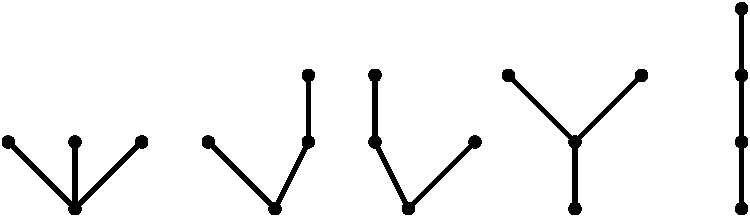
\includegraphics[scale=0.6]{Trees3}
\end{center}

Show that the number of plane trees on $n+1$ nodes is again the $n$\textsuperscript{th} Catalan number $\frac{1}{n+1}{2n \choose n}$, by 
finding a bijection to the number of unflooded routes to Bob. As a hint, below is shown two examples of the mapping given by a particular bijection $f$. (Your friendly TA will also provide another hint if asked...)

\begin{center}
    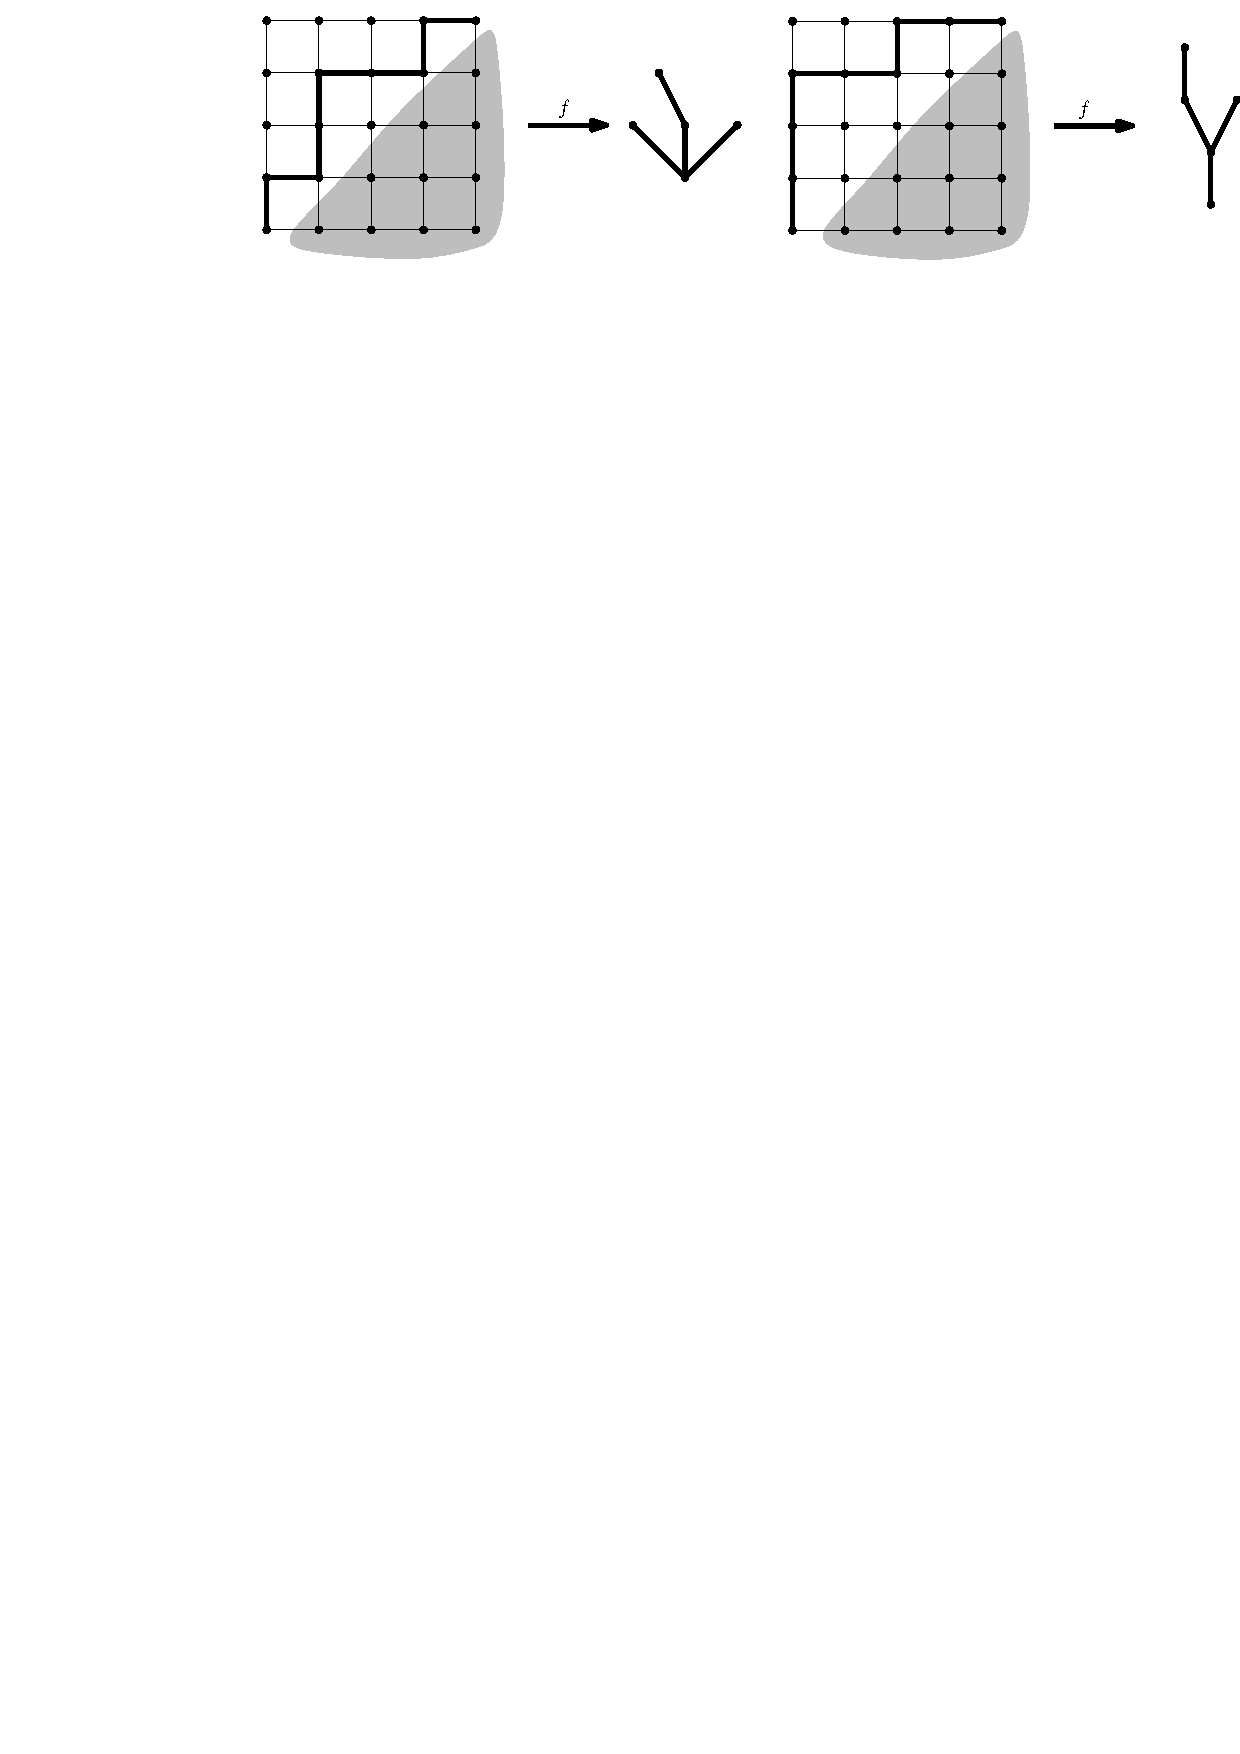
\includegraphics{flood2trees}
\end{center}

\solution{We define a mapping $f$ as follows. Imagine walking along the outside of a plane tree (keeping your right hand on the tree always), and construct a path from $(0,0)$ as follows. Each time you go away from the root, take a step north; each time you get closer to the root, take a step east. 

    This generates a path to $(n,n)$, since each edge is traversed once going up and once going down, so there will be a total of $n$ north steps and $n$ east steps. 
    Also, the path cannot visit a flooded intersection, since this would require that there is some $i$ so that in the first $i$ steps, there are more east steps than north steps; but this means taking more down steps than up steps in the tree, which would put you below the root!

    So the mapping $f$ is well defined from plane trees on $n+1$ nodes to unflooded paths to Bob. It is also an injection - two different trees will yield two distinct walks. Finally, it is a surjection: for any unflooded path to Bob, we can draw the corresponding plane tree; again, the restriction that we remain above the diagonal ensures that we're never asked to step down when we're at the root of the tree.

    So $f$ provides the required bijection.
}

\end{document}
